\documentclass[12pt,a4paper]{article}

% ─── Page Layout ───────────────────────────────────────────────────────────────
\usepackage[a4paper, margin=0.8in, headheight=14pt]{geometry}

% ─── Fonts (XeLaTeX) ───────────────────────────────────────────────────────────
\usepackage{fontspec}
\usepackage{unicode-math}
\setmainfont{TeX Gyre Pagella}
\setmonofont[Scale=0.88]{TeX Gyre Cursor}
\setmathfont{Latin Modern Math}

% ─── Packages ──────────────────────────────────────────────────────────────────
\usepackage{xcolor}
\usepackage{colortbl}
\usepackage{titlesec}
\usepackage{enumitem}
\usepackage{tabularx}
\usepackage{booktabs}
\usepackage{array}
\usepackage{amsmath}
\usepackage{tikz}
\usetikzlibrary{shapes.geometric, arrows.meta, positioning, calc, fit, decorations.pathreplacing, decorations.pathmorphing}
\usepackage{tcolorbox}
\tcbuselibrary{skins, breakable}
\usepackage{hyperref}
\usepackage{fancyhdr}
\usepackage{graphicx}
\usepackage{microtype}
\hyphenpenalty=10000
\exhyphenpenalty=10000
\sloppy
\usepackage{caption}
\usepackage{setspace}
\usepackage{multirow}
\usepackage{tocloft}

% ─── Q&A helper ────────────────────────────────────────────────────────────────
\newcommand{\Q}[1]{\textbf{#1}\par\noindent\ignorespaces}

% ─── Colour Palette ────────────────────────────────────────────────────────────
\definecolor{myred}{RGB}{196,30,58}
\definecolor{mydark}{RGB}{30,30,50}
\definecolor{mygreen}{RGB}{14,120,80}
\definecolor{myteal}{RGB}{0,130,140}
\definecolor{myamber}{RGB}{180,100,0}
\definecolor{mypurple}{RGB}{100,30,160}
\definecolor{mygray}{RGB}{246,247,249}
\definecolor{mgframe}{RGB}{180,185,200}
\definecolor{watermark}{RGB}{145,150,170}
\definecolor{hdrred}{RGB}{250,232,235}
\definecolor{hdrgreen}{RGB}{220,244,233}
\definecolor{hdrteal}{RGB}{220,242,244}
\definecolor{hdramber}{RGB}{253,242,215}
\definecolor{hdrpurple}{RGB}{238,228,255}
\definecolor{hdrgray}{RGB}{238,240,245}
\definecolor{rowalt}{RGB}{250,251,253}

% ─── Section Formatting ────────────────────────────────────────────────────────
\titleformat{\section}
  {\large\bfseries\color{myred}}{\thesection.}{0.5em}{}
  [\vspace{1pt}{\color{myred}\rule{\linewidth}{0.8pt}}]
\titleformat{\subsection}
  {\normalsize\bfseries\color{myteal}}{\thesubsection}{0.5em}{}
\titlespacing*{\section}{0pt}{18pt}{7pt}
\titlespacing*{\subsection}{0pt}{11pt}{4pt}

% ─── Paragraph ─────────────────────────────────────────────────────────────────
\setlength{\parindent}{0pt}
\setlength{\parskip}{4pt}

% ─── TOC Styling ───────────────────────────────────────────────────────────────
\renewcommand{\cfttoctitlefont}{\large\bfseries\color{myred}}
\renewcommand{\cftaftertoctitle}{\par\noindent{\color{myred}\rule{\linewidth}{0.8pt}}}
\setlength{\cftbeforetoctitleskip}{0pt}
\setlength{\cftaftertoctitleskip}{6pt}
\renewcommand{\cftsecfont}{\normalsize\bfseries\color{mydark}}
\renewcommand{\cftsecpagefont}{\normalsize\bfseries\color{mydark}}
\renewcommand{\cftsecleader}{\cftdotfill{\cftdotsep}}
\setlength{\cftbeforesecskip}{7pt}
\renewcommand{\cftsubsecfont}{\small\color{mydark}}
\renewcommand{\cftsubsecpagefont}{\small\color{mydark}}
\setlength{\cftbeforesubsecskip}{3pt}
\setlength{\cftsubsecindent}{1.4em}

% ─── Table helpers ─────────────────────────────────────────────────────────────
\renewcommand{\arraystretch}{1.45}
\setlength{\tabcolsep}{6pt}
\arrayrulecolor{mydark}
\newcolumntype{B}[1]{>{\small\bfseries\raggedright\arraybackslash}m{#1}}
\newcolumntype{C}[1]{>{\centering\arraybackslash}m{#1}}
\newcolumntype{Y}{>{\small\raggedright\arraybackslash}X}
\renewcommand{\tabularxcolumn}[1]{m{#1}}

% ─── Header / Footer ───────────────────────────────────────────────────────────
\pagestyle{fancy}
\fancyhf{}
\fancyhead[L]{\small\color{myred}\textbf{PE-EC703C}\;\color{mydark}--- Wavelet Transforms}
\fancyhead[R]{\small\color{myteal}\textbf{Module 1 Notes}}
\fancyfoot[C]{\small\color{mydark}\thepage}
\fancyfoot[R]{\small\color{watermark}\textit{\copyright\ Biraj Sarkar}}
\renewcommand{\headrulewidth}{0.5pt}
\renewcommand{\footrulewidth}{0.3pt}

% ─── Hyperref ──────────────────────────────────────────────────────────────────
\hypersetup{
  colorlinks=true, linkcolor=myteal, urlcolor=myteal,
  pdfauthor={Biraj Sarkar},
  pdftitle={PE-EC703C --- Module 1 Notes}
}

% ─── tcolorbox styles ──────────────────────────────────────────────────────────
\tcbset{
  tikzbox/.style={
    colback=mygray, colframe=mgframe, boxrule=0.6pt, arc=4pt,
    left=8pt, right=8pt, top=6pt, bottom=6pt,
    colbacktitle=mgframe, coltitle=mydark,
    fonttitle=\small\bfseries
  },
  defbox/.style={
    colback=hdrgreen, colframe=mygreen, boxrule=0.8pt, arc=4pt,
    left=9pt, right=9pt, top=6pt, bottom=6pt,
    colbacktitle=mygreen, coltitle=white,
    fonttitle=\small\bfseries
  },
  formulabox/.style={
    colback=hdrteal, colframe=myteal, boxrule=0.8pt, arc=4pt,
    left=9pt, right=9pt, top=7pt, bottom=7pt,
    colbacktitle=myteal, coltitle=white,
    fonttitle=\small\bfseries
  },
  examplebox/.style={
    colback=hdramber, colframe=myamber, boxrule=0.8pt, arc=4pt,
    left=9pt, right=9pt, top=6pt, bottom=6pt,
    colbacktitle=myamber, coltitle=white,
    fonttitle=\small\bfseries
  },
  masonbox/.style={
    colback=hdrpurple, colframe=mypurple, boxrule=0.8pt, arc=4pt,
    left=9pt, right=9pt, top=6pt, bottom=6pt,
    colbacktitle=mypurple, coltitle=white,
    fonttitle=\small\bfseries
  },
  exambox/.style={
    colback=hdrpurple, colframe=mypurple, boxrule=1pt, arc=5pt,
    left=10pt, right=10pt, top=8pt, bottom=8pt,
    colbacktitle=mypurple, coltitle=white,
    fonttitle=\bfseries,
    breakable, title after break={\textbf{Frequently Asked / Viva Questions (contd.)}}}
}
\tcbset{breakable}

% ─── TikZ styles ───────────────────────────────────────────────────────────────
\tikzset{
  block/.style={rectangle, draw=myteal, fill=hdrteal,
    text width=2.5cm, align=center, minimum height=1.0cm,
    font=\small, rounded corners=3pt, line width=0.7pt},
  redblock/.style={rectangle, draw=myred, fill=hdrred,
    text width=2.5cm, align=center, minimum height=1.0cm,
    font=\small, rounded corners=3pt, line width=0.7pt},
  arrow/.style={-Stealth, thick, color=mydark},
  redarrow/.style={-Stealth, thick, color=myred},
  line/.style={thick, color=mydark}
}

% ═══════════════════════════════════════════════════════════════════════════════
\begin{document}
% ═══════════════════════════════════════════════════════════════════════════════

\begin{center}
  {\LARGE\bfseries\color{myred} PE-EC703C --- Wavelet Transforms}\\[5pt]
  {\normalsize\color{mydark} Semester VII \quad$\bullet$\quad 3L:0T:0P \quad$\bullet$\quad 3 Credits}\\[3pt]
  {\normalsize\color{myteal}\textbf{Module 1 Exam Notes: Introduction to Wavelet Theory}}\\[3pt]
  {\small\color{mydark} CGEC \;$|$\; B.Tech ECE (2023--27) \;$|$\; \textit{Biraj Sarkar}}
\end{center}
\noindent{\color{myred}\rule{\linewidth}{1.5pt}}
\vspace{2pt}

\hypersetup{linkcolor=mydark}
\tableofcontents
\hypersetup{linkcolor=myteal}
\newpage

% ===============================================================================
\section{Introduction and Historical Development}
% ===============================================================================

\begin{tcolorbox}[defbox, title={\textbf{Definition of a Wavelet}}]
A \textbf{wavelet} is a localized, oscillatory wave-like function of effectively finite duration, with a zero mean value. Unlike a sine wave, which extends infinitely in both directions, a wavelet grows and decays over a short period, providing simultaneous \textbf{time} and \textbf{frequency} localization.
\end{tcolorbox}

\subsection{Historical Origin of Wavelets}
The development of wavelet theory is a synthesis of ideas spanning mathematics, physics, and digital signal processing:
\begin{itemize}[leftmargin=*, itemsep=3pt]
  \item \textbf{1910 (Alfréd Haar):} Proposed the first and simplest wavelet, the \textbf{Haar wavelet}, as an orthonormal basis for functions. It consists of a step function that changes value abruptly between $+1$ and $-1$.
  \item \textbf{1946 (Dennis Gabor):} Developed the Windowed Fourier Transform (or Gabor Transform) to introduce time localization using Gaussian window envelopes.
  \item \textbf{1981 (Jean Morlet):} A geophysicist processing seismic data introduced the concept of the "wavelet of constant shape" with variable scaling and translation to achieve depth resolution.
  \item \textbf{1984 (Alex Grossmann):} Collaborated with Morlet to establish the rigorous mathematical framework for the Continuous Wavelet Transform (CWT) using group theory.
  \item \textbf{1986 (Stéphane Mallat \& Yves Meyer):} Formulated \textbf{Multi-resolution Analysis (MRA)}, establishing a unified foundation connecting wavelets to subband digital filtering.
  \item \textbf{1988 (Ingrid Daubechies):} Constructed the first family of continuous, compactly supported, orthonormal wavelet bases with maximum vanishing moments (the \textbf{Daubechies wavelets}), making wavelets highly practical for computer implementation.
\end{itemize}

\subsection{Different Communities of Wavelet}
Wavelet theory is uniquely interdisciplinary, developed independently across multiple scientific domains:
\begin{enumerate}[leftmargin=*, itemsep=4pt]
  \item \textbf{Mathematics Community:} Studied under \textit{Calderón-Zygmund operators}, singular integrals, and harmonic analysis. Focuses on basis representations of Hilbert and Banach function spaces ($L^2(\mathbb{R})$).
  \item \textbf{Geophysics \& Physics Community:} Morlet and Grossmann used wavelets for seismic reflection parsing and quantum mechanics (coherent states, path integrals).
  \item \textbf{Digital Signal Processing (DSP) \& Engineering Community:} Developed wavelets as \textbf{filter banks} (subband coding) for audio, image, and video compression.
\end{enumerate}

% ===============================================================================
\section{Time-Frequency Analysis Limitations}
% ===============================================================================

Traditional signal analysis relies on the \textbf{Fourier Transform (FT)}, which maps a time-domain signal $x(t)$ to its frequency spectrum $X(f)$:
$$X(f) = \int_{-\infty}^{\infty} x(t) e^{-j 2\pi f t} dt$$

\begin{itemize}[leftmargin=*, itemsep=3.5pt]
  \item \textbf{Limitation:} FT has \textit{infinite time support} ($e^{-j 2\pi f t}$ spans from $-\infty$ to $\infty$). It yields perfect frequency resolution but completely destroys all time information (we know \textit{what} frequencies exist, but not \textit{when} they occur).
\end{itemize}

\subsection{Short-Time Fourier Transform (STFT)}
To introduce time localization, the \textbf{Short-Time Fourier Transform (STFT)} multiplies the signal with a sliding window function $w(t)$ centered at time $\tau$:
$$STFT_x(\tau, f) = \int_{-\infty}^{\infty} x(t) w^*(t - \tau) e^{-j 2\pi f t} dt$$

\begin{itemize}[leftmargin=*, itemsep=3.5pt]
  \item \textbf{Limitation:} The window width is \textbf{fixed} for all frequencies. 
  \item \textbf{Heisenberg's Uncertainty Principle:} The resolutions in time ($\Delta t$) and frequency ($\Delta f$) are bounded:
  $$\Delta t \cdot \Delta f \ge \frac{1}{4\pi}$$
  Under STFT, we must choose a fixed window. A narrow window gives good time resolution but poor frequency resolution (Wideband STFT). A wide window gives good frequency resolution but poor time resolution (Narrowband STFT).
\end{itemize}

\subsection{The Wavelet Multi-resolution Approach}
The Continuous Wavelet Transform (CWT) resolves this restriction by using a \textbf{variable-width window}:
\begin{itemize}[leftmargin=*, itemsep=3.5pt]
  \item At \textbf{high frequencies}, it uses narrow windows (high time resolution, lower frequency resolution) to capture rapid transients and edges.
  \item At \textbf{low frequencies}, it uses wide windows (high frequency resolution, lower time resolution) to capture slow-varying stationary components.
\end{itemize}

\newpage
\begin{tcolorbox}[tikzbox, title={Time-Frequency Tiling Grids Comparison}]
\centering
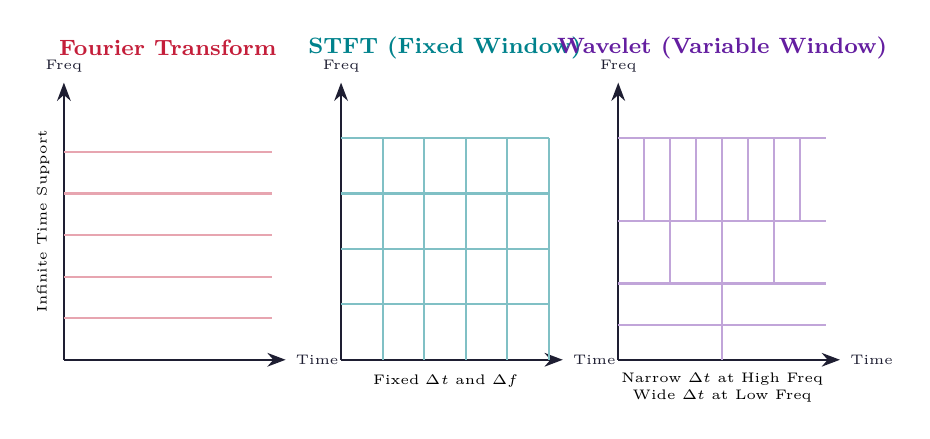
\begin{tikzpicture}[scale=0.88]
  % Fourier Transform Grid
  \node[font=\footnotesize\bfseries, color=myred] at (1.5,4.5) {Fourier Transform};
  \draw[arrow] (0,0) -- (3.2,0) node[right, font=\tiny] {Time};
  \draw[arrow] (0,0) -- (0,4) node[above, font=\tiny] {Freq};
  \foreach \x in {0.6, 1.2, 1.8, 2.4, 3.0} {
    \draw[line, color=myred!40] (0,\x) -- (3.0,\x);
  }
  \node[font=\tiny, rotate=90] at (-0.3, 2) {Infinite Time Support};

  % STFT Grid
  \node[font=\footnotesize\bfseries, color=myteal] at (5.5,4.5) {STFT (Fixed Window)};
  \draw[arrow] (4.0,0) -- (7.2,0) node[right, font=\tiny] {Time};
  \draw[arrow] (4.0,0) -- (4.0,4) node[above, font=\tiny] {Freq};
  \foreach \x in {0.8, 1.6, 2.4, 3.2} {
    \draw[line, color=myteal!50] (4.0,\x) -- (7.0,\x);
  }
  \foreach \y in {4.6, 5.2, 5.8, 6.4, 7.0} {
    \draw[line, color=myteal!50] (\y, 0) -- (\y, 3.2);
  }
  \node[font=\tiny] at (5.5, -0.3) {Fixed $\Delta t$ and $\Delta f$};

  % Wavelet Grid
  \node[font=\footnotesize\bfseries, color=mypurple] at (9.5,4.5) {Wavelet (Variable Window)};
  \draw[arrow] (8.0,0) -- (11.2,0) node[right, font=\tiny] {Time};
  \draw[arrow] (8.0,0) -- (8.0,4) node[above, font=\tiny] {Freq};
  
  % Dyadic divisions
  \draw[line, color=mypurple!40] (8.0, 0.5) -- (11.0, 0.5);
  \draw[line, color=mypurple!40] (8.0, 1.1) -- (11.0, 1.1);
  \draw[line, color=mypurple!40] (8.0, 2.0) -- (11.0, 2.0);
  \draw[line, color=mypurple!40] (8.0, 3.2) -- (11.0, 3.2);
  
  % Vertical lines
  \draw[line, color=mypurple!40] (9.5, 0) -- (9.5, 3.2);
  \draw[line, color=mypurple!40] (8.75, 1.1) -- (8.75, 3.2);
  \draw[line, color=mypurple!40] (10.25, 1.1) -- (10.25, 3.2);
  \draw[line, color=mypurple!40] (8.375, 2.0) -- (8.375, 3.2);
  \draw[line, color=mypurple!40] (9.125, 2.0) -- (9.125, 3.2);
  \draw[line, color=mypurple!40] (9.875, 2.0) -- (9.875, 3.2);
  \draw[line, color=mypurple!40] (10.625, 2.0) -- (10.625, 3.2);
  
  \node[font=\tiny, align=center] at (9.5, -0.4) {Narrow $\Delta t$ at High Freq\\Wide $\Delta t$ at Low Freq};
\end{tikzpicture}
\end{tcolorbox}

% ===============================================================================
\section{Classification of Continuous and Discrete Wavelet Transforms}
% ===============================================================================

Wavelet transforms are classified based on how the scaling parameter $a$ and translation parameter $b$ are sampled:

\begin{enumerate}[leftmargin=*, itemsep=4pt]
  \item \textbf{Continuous Wavelet Transform (CWT):} The parameters $a$ and $b$ vary continuously over $\mathbb{R} \setminus \{0\}$ and $\mathbb{R}$ respectively. This maps a 1D time-domain signal to a 2D time-scale plane, generating a highly redundant representation. It is ideal for signal analysis, singularity detection, and scientific research.
  \item \textbf{Discrete Wavelet Transform (DWT):} The parameters $a$ and $b$ are sampled discretely. Typically, a \textbf{dyadic grid} is used:
        $$a = 2^j, \quad b = k 2^j, \quad j, k \in \mathbb{Z}$$
        This eliminates representation redundancy, allowing for an orthogonal basis decomposition. It is highly efficient for data compression (e.g. JPEG 2000), denoising, and digital hardware implementation.
\end{enumerate}

\par\noindent
{\renewcommand{\arraystretch}{1.4}%
\begin{tabularx}{\linewidth}{|B{3.5cm}|Y|Y|}
\hline
\textbf{Feature} & \textbf{Continuous Wavelet (CWT)} & \textbf{Discrete Wavelet (DWT)} \\
\hline
\textbf{Scaling ($a$) \& Shift ($b$)} & Continuously variable ($a,b \in \mathbb{R}$). & Discretely sampled ($a=2^j, b=k2^j$). \\
\hline
\textbf{Redundancy} & High (infinite overlapping coefficients). & None (orthogonal / non-redundant). \\
\hline
\textbf{Reconstruction} & Uses stable double integral. & Uses digital filter banks (perfect reconstruction). \\
\hline
\textbf{Best Use Case} & Singularity parsing, physics, and analysis. & Signal compression, denoising, and coding. \\
\hline
\end{tabularx}}

% ===============================================================================
\section{Developments in Wavelet Theory Applications}
% ===============================================================================

Since its formalization, wavelet theory has seen rapid developments and applications across various engineering and scientific fields:
\begin{itemize}[leftmargin=*, itemsep=4pt]
  \item \textbf{Seismic Signal Processing:} Jean Morlet's initial development for processing geophysics reflection waves to localize underground oil deposits.
  \item \textbf{Data \& Image Compression:} Standardized in JPEG 2000 (DWT) and FBI fingerprint databases, allowing high-quality storage with minimal memory.
  \item \textbf{Biomedical Engineering:} Analyzing ECG (electrocardiogram) and EEG (electroencephalogram) signals for transient spike detection (such as epilepsy seizures) and denoising.
  \item \textbf{Communication Systems:} Subcarrier modulation schemes like Discrete Wavelet Multi-Tone (DWMT) to suppress inter-carrier interference in multicarrier systems.
\end{itemize}

\newpage
% ===============================================================================
\begin{center}
  {\large\bfseries\color{myred} Quick Revision --- Module 1}\\[3pt]
  {\small\color{mydark} Introduction to Wavelet Theory $|$ PE-EC703C}
\end{center}
\noindent{\color{myred}\rule{\linewidth}{1.2pt}}
\vspace{4pt}
% ===============================================================================

\begin{tcolorbox}[formulabox, title={\textbf{Key Time-Frequency Equations}}]
\renewcommand{\arraystretch}{1.35}
\begin{tabularx}{\linewidth}{B{5.0cm} X}
Fourier Transform & $X(f) = \int_{-\infty}^{\infty} x(t) e^{-j 2\pi f t} dt$ \\[4pt]
Short-Time FT (STFT) & $STFT_x(\tau, f) = \int_{-\infty}^{\infty} x(t) w^*(t - \tau) e^{-j 2\pi f t} dt$ \\[4pt]
Heisenberg Uncertainty & $\Delta t \cdot \Delta f \ge \frac{1}{4\pi} \quad$ (Limits simultaneous time-frequency resolution)
\end{tabularx}
\tcbset{after={\color{black}}}
\end{tcolorbox}

\begin{tcolorbox}[defbox, title={\textbf{One-Line Definitions}}]
\begin{itemize}[leftmargin=*, itemsep=3.5pt]
  \item \textbf{Wavelet:} A localized, oscillatory wave-like function of finite duration with a zero mean value.
  \item \textbf{Fourier Transform:} Spectral mapping with infinite time support, providing no temporal location details.
  \item \textbf{STFT:} Time-frequency mapping that uses a fixed window width, imposing rigid time-frequency resolutions.
  \item \textbf{Multi-resolution Approach:} Analysis method that analyzes signals with narrow windows at high frequencies and wide windows at low frequencies.
  \item \textbf{CWT:} Wavelet transform where parameters vary continuously, providing a redundant, high-resolution representation.
  \item \textbf{DWT:} Wavelet transform where parameters are sampled on a discrete grid, providing an orthogonal representation.
\end{itemize}
\end{tcolorbox}

\begin{tcolorbox}[exambox, title={\textbf{Frequently Asked / Viva Questions}}]
\begin{enumerate}[topsep=0pt, label=\textbf{Q\arabic*.}, itemsep=5pt]
  \item \Q{Why can the Fourier Transform not analyze non-stationary signals?}
        The Fourier Transform integrates over all time ($-\infty$ to $\infty$), meaning it assumes the signal's spectral components do not change over time. It has no time localization, so it cannot identify *when* a transient event or change in frequency occurs.

  \item \Q{How does the Short-Time Fourier Transform (STFT) attempt to fix the limitations of the Fourier Transform?}
        The STFT divides the signal into short segments by multiplying it with a sliding window function. The Fourier Transform is then computed for each segment, providing a time-frequency spectrogram.

  \item \Q{What is the drawback of the STFT?}
        The STFT uses a fixed window size for all frequencies. Due to Heisenberg's Uncertainty Principle ($\Delta t \cdot \Delta f \ge 1/4\pi$), a narrow window gives good time resolution but poor frequency resolution, while a wide window does the opposite.

  \item \Q{How do Wavelets resolve the resolution trade-off of the STFT?}
        Wavelets use variable-width windows: narrow windows (small scales) at high frequencies for capturing rapid transitions, and wide windows (large scales) at low frequencies for capturing steady long-term behaviors.

  \item \Q{What is the main difference between CWT and DWT in terms of redundancy and representation?}
        CWT translates and scales the mother wavelet continuously, leading to high redundancy and overlapping information, making it best for signal analysis. DWT samples parameters on a discrete dyadic grid, yielding a non-redundant orthogonal representation that is highly efficient for data compression.
\end{enumerate}
\end{tcolorbox}

\begin{tcolorbox}[tikzbox, title={\textbf{Time-Frequency Analysis Features}}]
\par\noindent
{\renewcommand{\arraystretch}{1.4}%
\begin{tabularx}{\linewidth}{|B{3.2cm}|Y|Y|Y|}
\hline
\textbf{Feature} & \textbf{Fourier Transform (FT)} & \textbf{Short-Time FT (STFT)} & \textbf{Wavelet Transform} \\
\hline
\textbf{Time Resolution} & None (integrates over all time). & Fixed (determined by window width). & Variable (excellent at high frequencies). \\
\hline
\textbf{Freq Resolution} & Perfect (at all frequencies). & Fixed (determined by window width). & Variable (excellent at low frequencies). \\
\hline
\textbf{Window Shape} & Infinite ($e^{-j 2\pi f t}$). & Fixed envelope ($w(t)$). & Scaled mother wavelet ($\psi(t/a)$). \\
\hline
\textbf{Best Use Case} & Stationary signals. & Quasi-stationary signals. & Non-stationary/transient signals. \\
\hline
\end{tabularx}}
\end{tcolorbox}

\end{document}
